\hypertarget{IndependenceTest_8c}{
\section{Independence\-Test.c File Reference}
\label{IndependenceTest_8c}\index{IndependenceTest.c@{IndependenceTest.c}}
}
{\tt \#include \char`\"{}party.h\char`\"{}}\par


Include dependency graph for Independence\-Test.c:\begin{figure}[H]
\begin{center}
\leavevmode
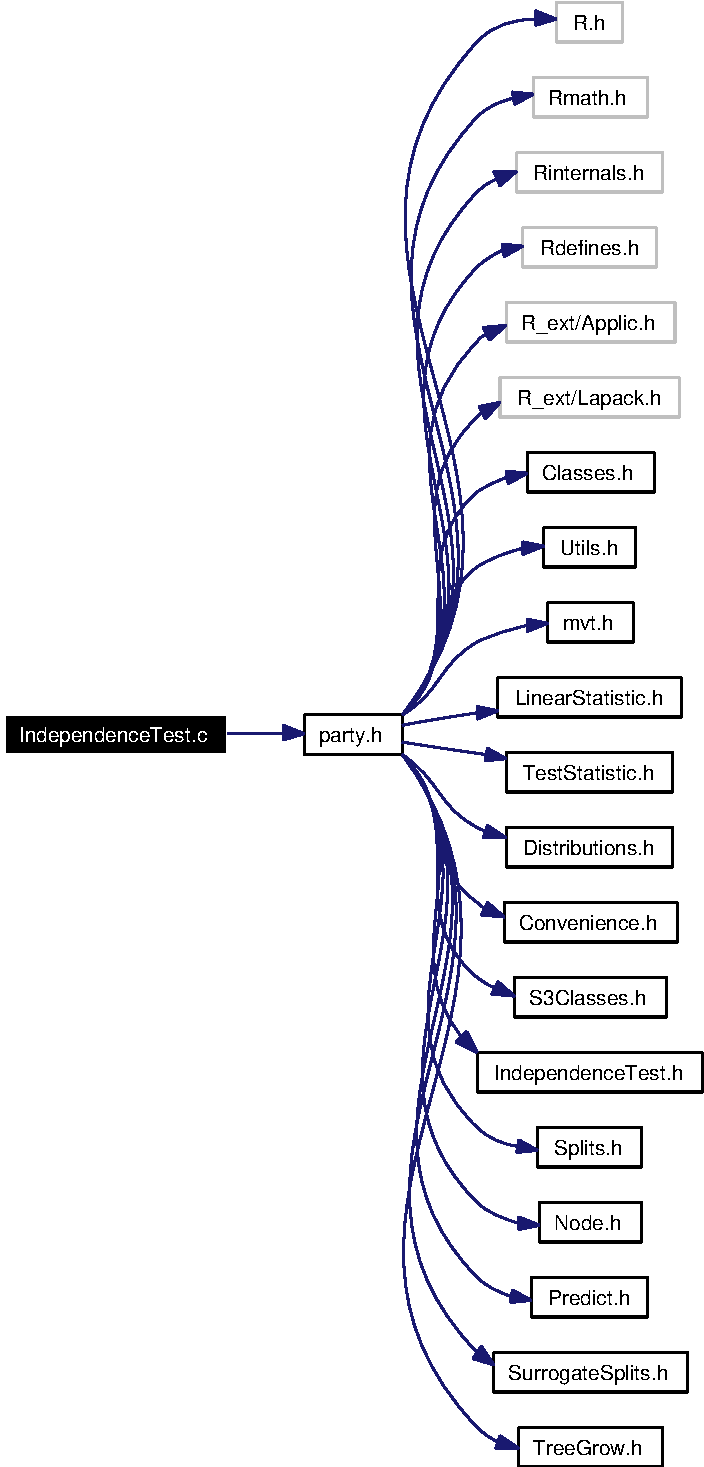
\includegraphics[width=186pt]{IndependenceTest_8c__incl}
\end{center}
\end{figure}
\subsection*{Functions}
\begin{CompactItemize}
\item 
void \hyperlink{IndependenceTest_8c_b02275a67ad210d96fed9864590ee3ef}{C\_\-Teststat\-Pvalue} (const SEXP linexpcov, const SEXP varctrl, double $\ast$ans\_\-teststat, double $\ast$ans\_\-pvalue)
\item 
void \hyperlink{IndependenceTest_8c_d33688ffc38df769a95d6964e5bb193a}{C\_\-Teststat\-Criterion} (const SEXP linexpcov, const SEXP varctrl, double $\ast$ans\_\-teststat, double $\ast$ans\_\-criterion)
\item 
void \hyperlink{IndependenceTest_8c_e64c8d91a58113cee43788dc1663d645}{C\_\-Independence\-Test} (const SEXP x, const SEXP y, const SEXP weights, SEXP linexpcov, SEXP varctrl, SEXP ans)
\item 
SEXP \hyperlink{IndependenceTest_8c_aab8e2db15687b6b95f802dd1719ed54}{R\_\-Independence\-Test} (SEXP x, SEXP y, SEXP weights, SEXP linexpcov, SEXP varctrl)
\item 
void \hyperlink{IndependenceTest_8c_0de2357bd1d38058c0cfc68c3e743b34}{C\_\-Global\-Test} (const SEXP learnsample, const SEXP weights, SEXP fitmem, const SEXP varctrl, const SEXP gtctrl, const double minsplit, double $\ast$ans\_\-teststat, double $\ast$ans\_\-criterion)
\item 
SEXP \hyperlink{IndependenceTest_8c_f80dcff3dd9196b9f861fd83f4efa8ac}{R\_\-Global\-Test} (SEXP learnsample, SEXP weights, SEXP fitmem, SEXP varctrl, SEXP gtctrl)
\end{CompactItemize}


\subsection{Detailed Description}
Functions for variable selection in each node of a tree

\begin{Desc}
\item[Author:]\begin{Desc}
\item[Author]hothorn \end{Desc}
\end{Desc}
\begin{Desc}
\item[Date:]\begin{Desc}
\item[Date]2007-02-02 11:22:45 +0100 (Fri, 02 Feb 2007) \end{Desc}
\end{Desc}


Definition in file \hyperlink{IndependenceTest_8c-source}{Independence\-Test.c}.

\subsection{Function Documentation}
\hypertarget{IndependenceTest_8c_0de2357bd1d38058c0cfc68c3e743b34}{
\index{IndependenceTest.c@{Independence\-Test.c}!C_GlobalTest@{C\_\-GlobalTest}}
\index{C_GlobalTest@{C\_\-GlobalTest}!IndependenceTest.c@{Independence\-Test.c}}
\subsubsection[C\_\-GlobalTest]{\setlength{\rightskip}{0pt plus 5cm}void C\_\-Global\-Test (const SEXP {\em learnsample}, const SEXP {\em weights}, SEXP {\em fitmem}, const SEXP {\em varctrl}, const SEXP {\em gtctrl}, const double {\em minsplit}, double $\ast$ {\em ans\_\-teststat}, double $\ast$ {\em ans\_\-criterion})}}
\label{IndependenceTest_8c_0de2357bd1d38058c0cfc68c3e743b34}


Perform a global test on independence of a response and multiple inputs \par
 \begin{Desc}
\item[Parameters:]
\begin{description}
\item[{\em learnsample}]an object of class `Learning\-Sample' \item[{\em weights}]case weights \item[{\em fitmem}]an object of class `Tree\-Fit\-Memory' \item[{\em varctrl}]an object of class `Variable\-Control' \item[{\em gtctrl}]an object of class `Global\-Test\-Control' \item[{\em minsplit}]minimum sum of weights to proceed \item[{\em ans\_\-teststat}]return value; vector of test statistics \item[{\em ans\_\-criterion}]return value; vector of node criteria (adjusted) pvalues or raw test statistics \end{description}
\end{Desc}


Definition at line 129 of file Independence\-Test.c.

References C\_\-Expect\-Covar\-Influence(), get\_\-ninputs(), get\_\-nobs(), get\_\-test\_\-trafo(), ncol(), PL2\_\-expcovinf\-Sym, PL2\_\-inputs\-Sym, PL2\_\-responses\-Sym, and PL2\_\-sumweights\-Sym.

Referenced by C\_\-Node(), and R\_\-Global\-Test().

Here is the call graph for this function:\begin{figure}[H]
\begin{center}
\leavevmode
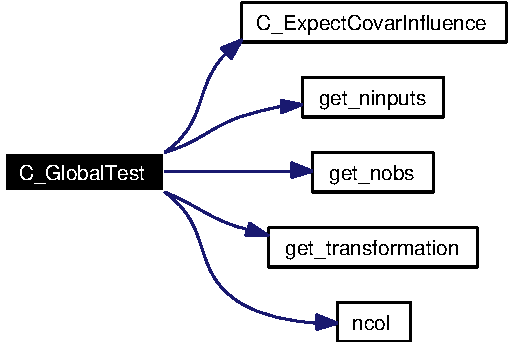
\includegraphics[width=139pt]{IndependenceTest_8c_0de2357bd1d38058c0cfc68c3e743b34_cgraph}
\end{center}
\end{figure}
\hypertarget{IndependenceTest_8c_e64c8d91a58113cee43788dc1663d645}{
\index{IndependenceTest.c@{Independence\-Test.c}!C_IndependenceTest@{C\_\-IndependenceTest}}
\index{C_IndependenceTest@{C\_\-IndependenceTest}!IndependenceTest.c@{Independence\-Test.c}}
\subsubsection[C\_\-IndependenceTest]{\setlength{\rightskip}{0pt plus 5cm}void C\_\-Independence\-Test (const SEXP {\em x}, const SEXP {\em y}, const SEXP {\em weights}, SEXP {\em linexpcov}, SEXP {\em varctrl}, SEXP {\em ans})}}
\label{IndependenceTest_8c_e64c8d91a58113cee43788dc1663d645}


Test of independence between x and y \par
 \begin{Desc}
\item[Parameters:]
\begin{description}
\item[{\em x}]values of the transformation \item[{\em y}]values of the influence function \item[{\em weights}]case weights \item[{\em linexpcov}]an object of class `Variable\-Control' for T \item[{\em varctrl}]an object of class `Variable\-Control' \item[{\em ans;}]return value, a double vector (teststat, pvalue) \end{description}
\end{Desc}


Definition at line 78 of file Independence\-Test.c.

References C\_\-Lin\-Stat\-Exp\-Cov(), C\_\-Lin\-Stat\-Exp\-Cov\-MPinv(), C\_\-Teststat\-Pvalue(), get\_\-teststat(), get\_\-tol(), ncol(), nrow(), and PL2\_\-expcovinf\-Sym.

Referenced by R\_\-Independence\-Test().

Here is the call graph for this function:\begin{figure}[H]
\begin{center}
\leavevmode
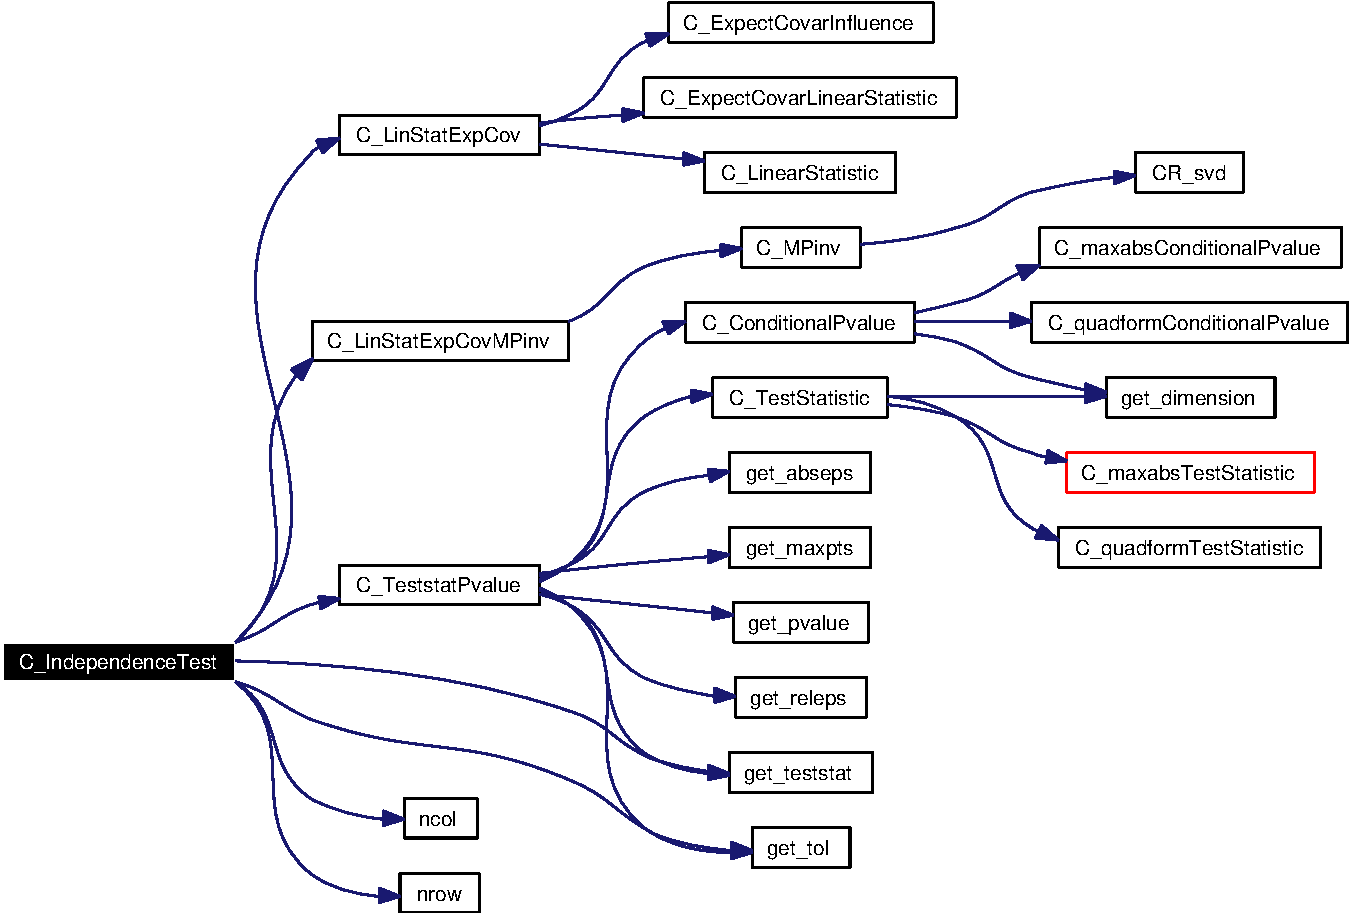
\includegraphics[width=341pt]{IndependenceTest_8c_e64c8d91a58113cee43788dc1663d645_cgraph}
\end{center}
\end{figure}
\hypertarget{IndependenceTest_8c_d33688ffc38df769a95d6964e5bb193a}{
\index{IndependenceTest.c@{Independence\-Test.c}!C_TeststatCriterion@{C\_\-TeststatCriterion}}
\index{C_TeststatCriterion@{C\_\-TeststatCriterion}!IndependenceTest.c@{Independence\-Test.c}}
\subsubsection[C\_\-TeststatCriterion]{\setlength{\rightskip}{0pt plus 5cm}void C\_\-Teststat\-Criterion (const SEXP {\em linexpcov}, const SEXP {\em varctrl}, double $\ast$ {\em ans\_\-teststat}, double $\ast$ {\em ans\_\-criterion})}}
\label{IndependenceTest_8c_d33688ffc38df769a95d6964e5bb193a}


Computes the test statistic and the node criterion \par
 \begin{Desc}
\item[Parameters:]
\begin{description}
\item[{\em linexpcov}]an object of class `Lin\-Stat\-Expect\-Covar' \item[{\em varctrl}]an object of class `Variable\-Control' \item[{\em ans\_\-teststat;}]return value, the test statistic \item[{\em ans\_\-criterion;}]return value, thep-value \end{description}
\end{Desc}


Definition at line 53 of file Independence\-Test.c.

References C\_\-Teststat\-Pvalue(), and get\_\-pvalue().

Here is the call graph for this function:\begin{figure}[H]
\begin{center}
\leavevmode
\includegraphics[width=370pt]{IndependenceTest_8c_d33688ffc38df769a95d6964e5bb193a_cgraph}
\end{center}
\end{figure}
\hypertarget{IndependenceTest_8c_b02275a67ad210d96fed9864590ee3ef}{
\index{IndependenceTest.c@{Independence\-Test.c}!C_TeststatPvalue@{C\_\-TeststatPvalue}}
\index{C_TeststatPvalue@{C\_\-TeststatPvalue}!IndependenceTest.c@{Independence\-Test.c}}
\subsubsection[C\_\-TeststatPvalue]{\setlength{\rightskip}{0pt plus 5cm}void C\_\-Teststat\-Pvalue (const SEXP {\em linexpcov}, const SEXP {\em varctrl}, double $\ast$ {\em ans\_\-teststat}, double $\ast$ {\em ans\_\-pvalue})}}
\label{IndependenceTest_8c_b02275a67ad210d96fed9864590ee3ef}


Computes the test statistic and, if requested, the corresponding P-value for a linear statistic \par
 \begin{Desc}
\item[Parameters:]
\begin{description}
\item[{\em linexpcov}]an object of class `Lin\-Stat\-Expect\-Covar' \item[{\em varctrl}]an object of class `Variable\-Control' \item[{\em ans\_\-teststat;}]return value, the test statistic \item[{\em ans\_\-pvalue;}]return value, the p-value \end{description}
\end{Desc}


Definition at line 21 of file Independence\-Test.c.

References C\_\-Conditional\-Pvalue(), C\_\-Test\-Statistic(), get\_\-abseps(), get\_\-maxpts(), get\_\-pvalue(), get\_\-releps(), get\_\-teststat(), and get\_\-tol().

Referenced by C\_\-Independence\-Test(), and C\_\-Teststat\-Criterion().

Here is the call graph for this function:\begin{figure}[H]
\begin{center}
\leavevmode
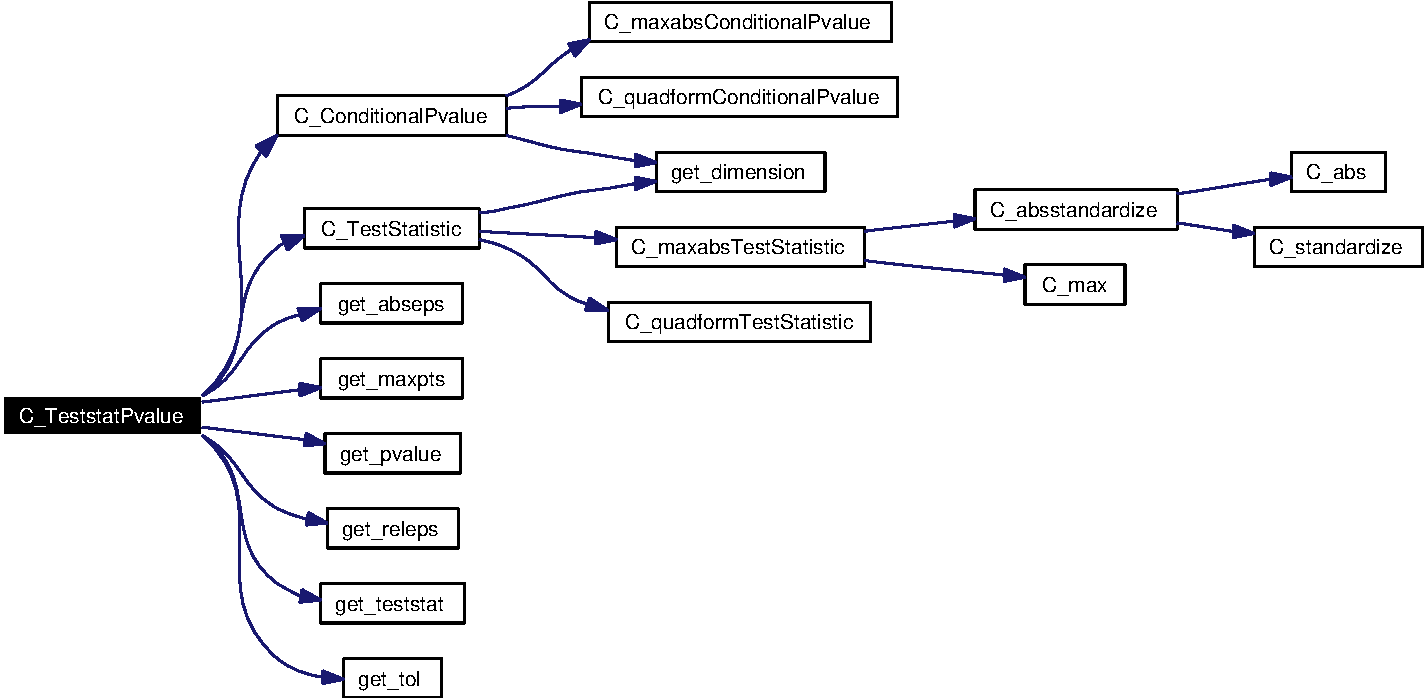
\includegraphics[width=359pt]{IndependenceTest_8c_b02275a67ad210d96fed9864590ee3ef_cgraph}
\end{center}
\end{figure}
\hypertarget{IndependenceTest_8c_f80dcff3dd9196b9f861fd83f4efa8ac}{
\index{IndependenceTest.c@{Independence\-Test.c}!R_GlobalTest@{R\_\-GlobalTest}}
\index{R_GlobalTest@{R\_\-GlobalTest}!IndependenceTest.c@{Independence\-Test.c}}
\subsubsection[R\_\-GlobalTest]{\setlength{\rightskip}{0pt plus 5cm}SEXP R\_\-Global\-Test (SEXP {\em learnsample}, SEXP {\em weights}, SEXP {\em fitmem}, SEXP {\em varctrl}, SEXP {\em gtctrl})}}
\label{IndependenceTest_8c_f80dcff3dd9196b9f861fd83f4efa8ac}


R-interface to C\_\-Global\-Test \par
 \begin{Desc}
\item[Parameters:]
\begin{description}
\item[{\em learnsample}]an object of class `Learning\-Sample' \item[{\em weights}]case weights \item[{\em fitmem}]an object of class `Tree\-Fit\-Memory' \item[{\em varctrl}]an object of class `Variable\-Control' \item[{\em gtctrl}]an object of class `Global\-Test\-Control' \end{description}
\end{Desc}


Definition at line 277 of file Independence\-Test.c.

References C\_\-Global\-Test(), and get\_\-ninputs().

Here is the call graph for this function:\begin{figure}[H]
\begin{center}
\leavevmode
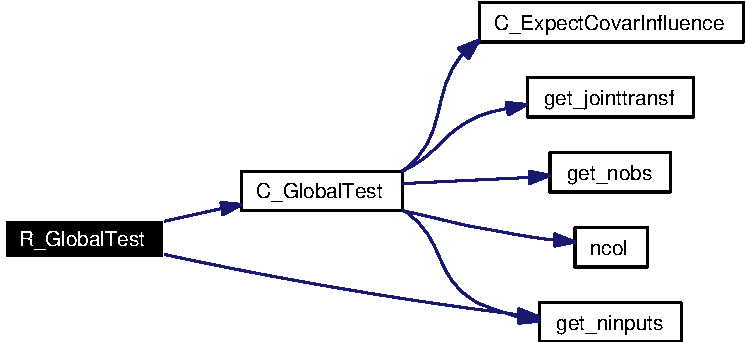
\includegraphics[width=196pt]{IndependenceTest_8c_f80dcff3dd9196b9f861fd83f4efa8ac_cgraph}
\end{center}
\end{figure}
\hypertarget{IndependenceTest_8c_aab8e2db15687b6b95f802dd1719ed54}{
\index{IndependenceTest.c@{Independence\-Test.c}!R_IndependenceTest@{R\_\-IndependenceTest}}
\index{R_IndependenceTest@{R\_\-IndependenceTest}!IndependenceTest.c@{Independence\-Test.c}}
\subsubsection[R\_\-IndependenceTest]{\setlength{\rightskip}{0pt plus 5cm}SEXP R\_\-Independence\-Test (SEXP {\em x}, SEXP {\em y}, SEXP {\em weights}, SEXP {\em linexpcov}, SEXP {\em varctrl})}}
\label{IndependenceTest_8c_aab8e2db15687b6b95f802dd1719ed54}


R-interface to C\_\-Independence\-Test \par
 \begin{Desc}
\item[Parameters:]
\begin{description}
\item[{\em x}]values of the transformation \item[{\em y}]values of the influence function \item[{\em weights}]case weights \item[{\em linexpcov}]an object of class `Variable\-Control' for T \item[{\em varctrl}]an object of class `Variable\-Control' \end{description}
\end{Desc}


Definition at line 105 of file Independence\-Test.c.

References C\_\-Independence\-Test().

Here is the call graph for this function:\begin{figure}[H]
\begin{center}
\leavevmode
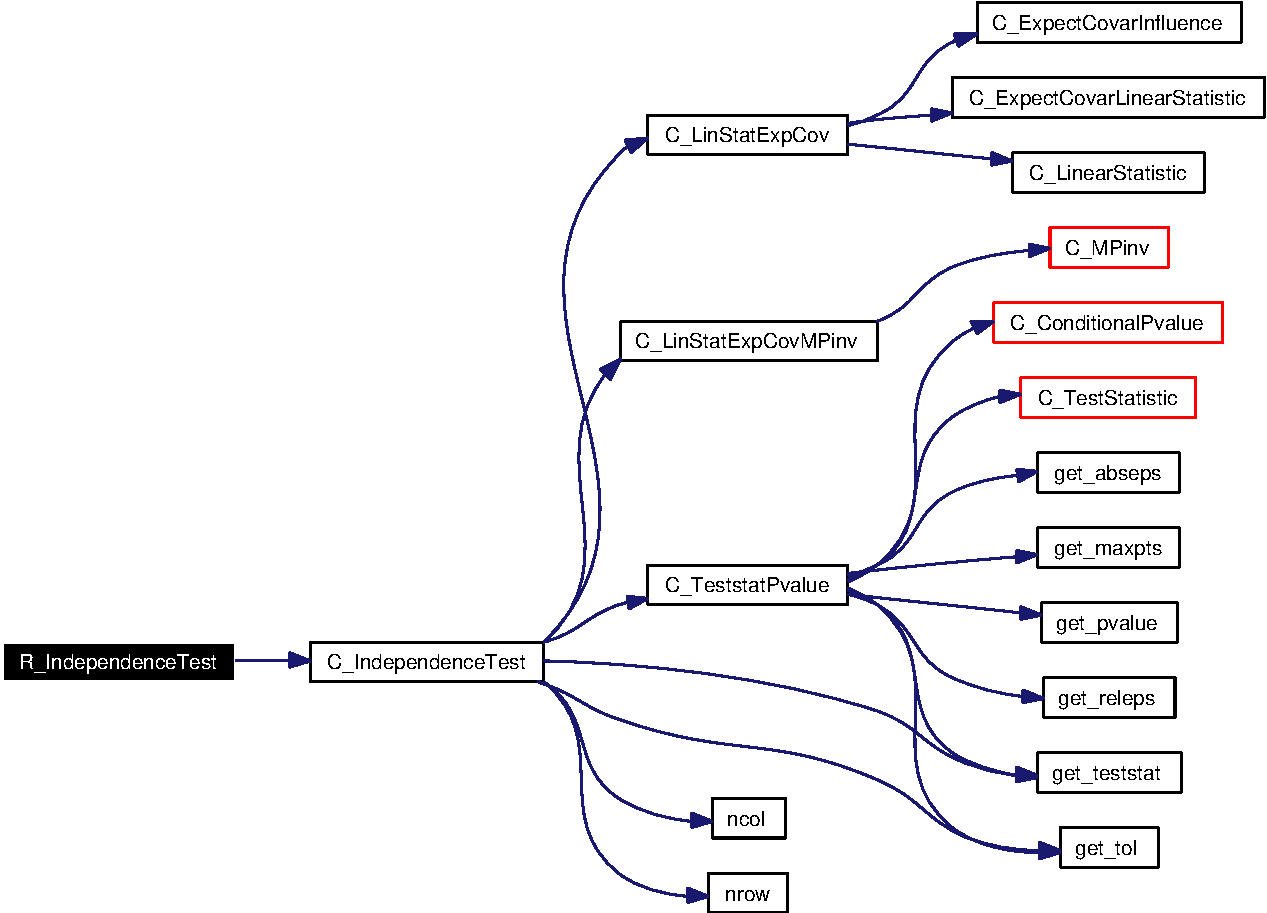
\includegraphics[width=321pt]{IndependenceTest_8c_aab8e2db15687b6b95f802dd1719ed54_cgraph}
\end{center}
\end{figure}
